\documentclass[a4paper, 10pt, twocolumn]{article} 
\setlength{\columnsep}{5mm}
\usepackage[left=1cm, top=1cm, bottom=2cm, right=1cm]{geometry}
\usepackage{amsthm}
\usepackage{amsmath}
\usepackage{amssymb} 
\usepackage[fleqn]{mathtools}
\usepackage{xcolor}
\definecolor{umblue}{HTML}{00274C}
\definecolor{ummaize}{HTML}{FFCB05}
\usepackage{graphicx} 
\usepackage{url}			       
\usepackage{hyperref}
\usepackage{pgf}
\usepackage{tikz}
\usetikzlibrary{arrows,automata}

% \pagestyle{empty} %

\date{\today} %

\def\keywords#1{\begin{center}{\bf Keywords}\\{#1}\end{center}} %

% Please, do not change any of the above lines

\tolerance=1
\emergencystretch=\maxdimen
\hyphenpenalty=10000
\hbadness=10000

\newcommand{\XB}{\color{black}}
\newcommand{\XBB}{\color{blue}}
\newcommand{\XV}{\color{violet}}
\newcommand{\XR}{\color{red}}

\newcommand{\ds}{\displaystyle}


\begin{document}

% Type down your paper title
\title{MTH 402 CAPSTONE \\ COMMUNITY DETECTION IN NETWORKS}

\vspace{0.25cm}
% Authors
\author{Cason Konzer  \\ %
       University of Michigan - Flint \\ % Affiliation 1
       % Add authors and affiliation as needed 
       \textit{ \color{violet}
       \href{mailto:casonk@umich.edu}{casonk@umich.edu}}  % Only one corresponding e-mail
       }%

\twocolumn[
\begin{@twocolumnfalse}

\maketitle

% \thispagestyle{empty}

% The abstract


\begin{abstract}

Network analysis is a growing field of study in Mathematics, Computer and Data Science. 
In the past decades many advances have been made in algorithm development and computational power. 
Applications of network analysis have spread wide across many fields, some interesting examples include supply chain, social media, author citation and web page networks. 
In the this paper we start by reviewing motivations for community detection in networks, and what defines well selected communities.
To do so we discuss papers in theory, and in application, while supplementing network basics required. 
We conclude by reviewing the development of community detection algorithms, and an in depth view of select a few. 

\end{abstract}

\keywords{Communities, Networks, Social Media} % Write down at least 3 Keywords

\end{@twocolumnfalse}
]


\section{Introduction}

Within mathematics, there are certain esteemed historical problems widely taught and know by those studying the field. 
To reminisce for a moment, I was introduced to two of these problems in my discrete mathematics class while in my second semester of undergraduate education. 
The seven bridges of Königsberg and the travelling salesman problem, both problems are prominent in graph theory.
Both of these problems can be easily visualized, land masses connected by bridges and cities by roads, map reading is instilled within common human culture. 
In a similar manner a graph represented by nodes connected by edges is intuitive while scale is small. 
We can represent so much in this format, infrastructure, relationships, information flow, etc. 
Once networks become large, visualization and intuition fall off, and abstracts allow for greater understanding. 

In a brief overview of the study of networks \cite{struc_funct_cnets}, Newman focuses on real world network types, properties of networks, null graph models and processes taking place on networks. 
The study of networks in general, has drawn initial attention by mathematicians, but in the recent century, and moreover the recent decades, computer and data scientists alike have been having a field day with their applications. 
Within the even more recent years, the study of (social) media networks has grown rapidly. 
Individuals are being persuaded by bots, Trump is banned from twitter while president, and idealogies are becoming seemingly more radicalized. 
Communities can be though of as densely connected groups of users of which have sparse, or otherwise less dense, connections to other groups \cite{com_struct_in_soc_and_bio}.
Why would industry care about such a community detection algorithm? 
Consider platforms such as Netflix or Amazon, recommender systems suggest products to a user. 
Similarly, consider radicalized or terrorist groups acting on cellular networks. 
In either case, one way we might identify similar products / individuals to others is by finding the community in which they reside. 
Community detection and clustering is an interesting approach to tackle these issues, what if we could identify profitable products, bot nets and radicalized individuals, or predict attacks by leveraging network structure?

In 2002 Girvan and Newman introduced the network community detection nomenclature shifting from previous definitions of network clustering \cite{com_struct_in_soc_and_bio}. 
In 2008 the Louvain algorithm \cite{louvain} for detecting communities within networks was published, and has become increasingly popular due to its advantageous run time. 
Additionally, the algorithm was shortly after extended to directed networks, akin to many media networks, and to include a `resolution' parameter \cite{louvain_resolution, com_struct_indir} providing the ability to tune for community size / density. 
Lesser known, Clauset, Newman, and Moore laid the underlying mathematics in 2004 \cite{finding_comm_struct}, Newman then extended this to weighted networks soon after \cite{analysis_of_wnets}. 
Additional community detections methods have emerged since, for example the Leiden \cite{louvain_2_leiden} and BigCLAM \cite{bigclam} algorithms. 
What is common among many of these algorithms is their way of scoring the goodness of community partitions. 
In 2003 Newman proposed the metric so called modularity leveraging the number of inter-community edges in comparison to the expectation \cite{finding_and_evaling_comm_struct}.
No matter the method, detecting communities is only an initial step to any research effort in media networks. 
To be of relevance, communities must be labeled in a meaningful way, and further their characteristics must be reviewed. 

This type of study has been of persistent interest within the social sciences. 
In the late 80s Krackhardt and Stern \cite{inet_crises} leveraged their university positions to study group dynamics of organizations via student assignments. 
A brief summary of their results finds that organizations which extend their reach externally performed superiorly. 
The so called `EI-Index' was developed as a key metric measuring the relationship between internal and external links. 
`Echochambers' and `Filter Bubbles' have become common words within the literature, and studies on media networks such as Twitter, Facebook, and Reddit \cite{eko_weko, sm_ece, ekoin_ekobtwin} are now commonplace. 
The effects of community structure and internet use in general has sparked similar research in sociology \cite{antisocial, eko_and_episteme, conspiracies_online, captivating}, and become of an increased political interest with rising concerns of impacts on today's youth. 
A thorough understanding of the structure of networks, community detection algorithms, and community analysis make for a optimistic outlook on solving societal problems stemming from media networks.


\section{Network Basics}

For ease of future discussion, let us set now some nomenclature and consider some of the first key features of networks. 
Common within literature there are two ways to refer to each of the two main ingredients of a network. 
Nodes, or vertices, are the crucial element of networks. 
These are users within media networks, web pages in the World Wide Web, species in food webs, and intersections or hubs in transit networks. 
On the other hand we have edges, or links, which are the glue holding nodes together and explaining their interaction. 
Within media networks these represent interactions such as friendships, likes, reposts, or comments. 
For the World Wide Web these are hyperlinks, references, or pointers from webpage to webpage.
In the study of food webs edges represent the predator prey relationship, and within transit networks the roads, railways, or routes themselves. 

Following standard, we denote $ n $ to be the number of nodes in the network, and $ m $ the number of edges. 
Similarly, we will denote $ k_i $ as the degree of node $ i $. 
The degree of a node is equal to the number of edges incident on it.
Edges can be mutual, or undirected, such that an edge between node $ i $ and $ j $ is just that. 
Also edges can be weighted, one may think of weighted edges in the example of food webs as the proportion of a species diet, or within roads as the number of lanes. 
Last edges can be directed, for example a web-link from on page to another, or a one-way street joining two intersections.
Within directed networks we derive two types of node degree, in-degree and out-degree, of which we will denote $ k_{i}^{in} $ and $ k_{i}^{out} $ for a node $ i $ respectively.
In-degree represents the number of inbound directed edges incident upon a node, and out-degree the number of edges originating from a node. 
We have thus the constraint that $ k_{i}^{in} + k_{i}^{out} = k_{i} $, or that a node's total degree is the sum of it's in and out degree. 
In the study of real world networks, one will find common all of these edge attributes within a single graph.
In the development of community detection algorithms, each feature requires an additional effort to implement. 

\begin{figure}[b]
       \centering
       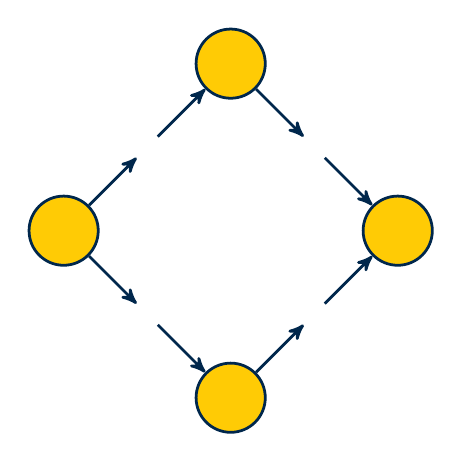
\begin{tikzpicture}[->,>=stealth',auto,node distance=1.5cm,semithick,line width=1pt]
              \tikzstyle{every state}=[fill=ummaize,draw=umblue,text=white]
              \tikzstyle{mid}=[fill=white,draw=none,text=white]
              \tikzstyle{e}=[color=umblue]
              
              \node[state]         (A)                     {};
              \node[mid]          (AB)  [above right of=A] {};
              \node[state]         (B) [above right of=AB] {};
              \node[mid]          (AC)  [below right of=A] {};
              \node[state]         (C) [below right of=AC] {};
              \node[mid]          (BD)  [below right of=B] {};
              \node[state]         (D) [below right of=BD] {};
              \node[mid]          (CD)   [below left of=D] {};
              \node[mid]          (AD)         [left of=D] {};
              
              \path  (A)  edge[e]              node {} (AB)
                     (AB) edge[e]              node {} (B)
                     (A)  edge[e]              node {} (AC)
                     (AC) edge[e]              node {} (C)
                     (B)  edge[e]              node {} (BD)
                     (BD) edge[e]              node {} (D)
                     (C)  edge[e]              node {} (CD)
                     (CD) edge[e]              node {} (D);
              
       \end{tikzpicture}
       \caption{Spoke Representation}
       \label{fig:spokes}
\end{figure}    

It is useful now to introduce the configuration model, of which is described in depth by Newman in \cite{networks}. 
Under this model each node has a know degree, as is often the case in network data set.  
As each edge is incident upon two nodes, it follows closely that summing degree across all nodes should be twice that the number of edges within the network : $ \sum_{i}^{n} k_{i} = 2m $.
For here a useful visualization is provided in Figure ~\ref{fig:spokes}, such that we view each node as depicted with spokes representing their edge connections. 
For the remainder of this paper we will denote $ s $ as the number of spokes, or twice the number of edges, within a network. 

A standard representation of networks is via an adjacency matrix, denoted $ A $. 
The entry $ A_{i,j} $ represents the number of edges from node $ i $ to node $ j $. 
A practical way to represent weighted networks is let the weights correspond to the number of edges, in the case of non-integer weights, a scaling can be applied by the greatest common factor to transform the matrix into one with integer only entries. 
In undirected networks, adjacency matrices exhibit symmetry across the diagonal, denoted $ \vec{A} $. 
For the given network in Figure ~\ref{fig:ex_network}, we see the following directed adjacency matrix, $ A $.

\begin{center}
       \begin{tabular}{c|ccccccc} 
              $ \vec{A} $ & $ a $ & $ b $ & $ c $ & $ d $ & $ e $ & $ f $ & $ g $ \\
              \hline
              $ a $ & $ 1 $ & $ 0 $ & $ 0 $ & $ 1 $ & $ 1 $ & $ 0 $ & $ 0 $ \\
              $ b $ & $ 0 $ & $ 1 $ & $ 1 $ & $ 0 $ & $ 0 $ & $ 1 $ & $ 0 $ \\
              $ c $ & $ 0 $ & $ 0 $ & $ 0 $ & $ 0 $ & $ 1 $ & $ 0 $ & $ 1 $ \\
              $ d $ & $ 1 $ & $ 0 $ & $ 0 $ & $ 1 $ & $ 0 $ & $ 0 $ & $ 0 $ \\
              $ e $ & $ 1 $ & $ 0 $ & $ 0 $ & $ 1 $ & $ 0 $ & $ 0 $ & $ 0 $ \\
              $ f $ & $ 0 $ & $ 0 $ & $ 1 $ & $ 0 $ & $ 0 $ & $ 1 $ & $ 1 $ \\
              $ g $ & $ 0 $ & $ 1 $ & $ 1 $ & $ 0 $ & $ 0 $ & $ 0 $ & $ 1 $ \\
       \end{tabular}
\end{center}

\noindent
Similarly if we consider Figure ~\ref{fig:ex_network} as an undirected graph, we have the symmetric adjacency matrix.

\begin{center}
       \begin{tabular}{c|ccccccc} 
              $ A $ & $ a $ & $ b $ & $ c $ & $ d $ & $ e $ & $ f $ & $ g $ \\
              \hline
              $ a $ & $ 1 $ & $ 0 $ & $ 0 $ & $ 2 $ & $ 1 $ & $ 0 $ & $ 0 $ \\
              $ b $ & $ 0 $ & $ 1 $ & $ 1 $ & $ 0 $ & $ 0 $ & $ 1 $ & $ 1 $ \\
              $ c $ & $ 0 $ & $ 1 $ & $ 0 $ & $ 0 $ & $ 1 $ & $ 1 $ & $ 2 $ \\
              $ d $ & $ 2 $ & $ 0 $ & $ 0 $ & $ 1 $ & $ 1 $ & $ 0 $ & $ 0 $ \\
              $ e $ & $ 1 $ & $ 0 $ & $ 1 $ & $ 1 $ & $ 0 $ & $ 0 $ & $ 0 $ \\
              $ f $ & $ 0 $ & $ 1 $ & $ 1 $ & $ 0 $ & $ 0 $ & $ 1 $ & $ 1 $ \\
              $ g $ & $ 0 $ & $ 1 $ & $ 2 $ & $ 0 $ & $ 0 $ & $ 1 $ & $ 1 $ \\
       \end{tabular}
\end{center}

\begin{figure}[t]
       \centering
       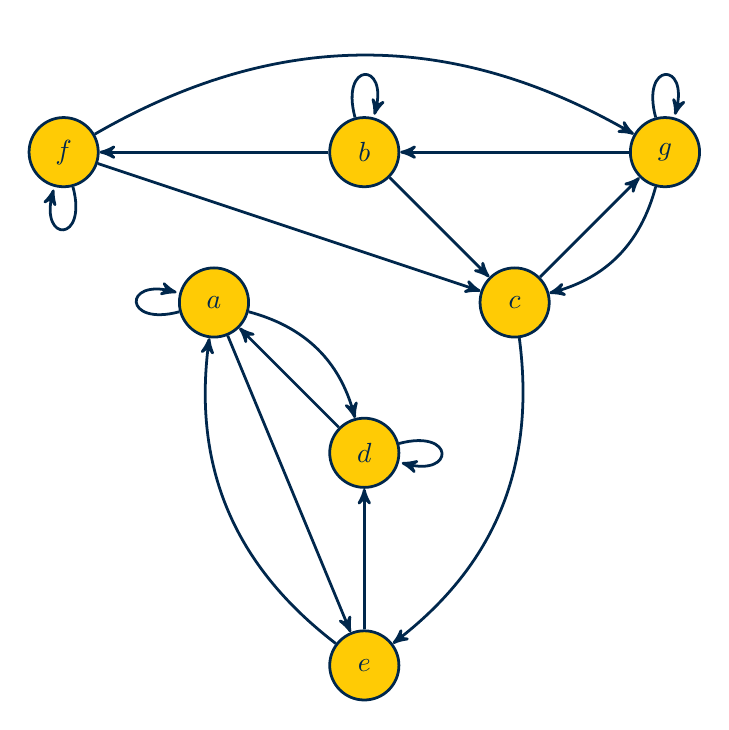
\begin{tikzpicture}[->,>=stealth',auto,node distance=2.7cm,semithick,line width=1pt]
              \tikzstyle{every state}=[fill=ummaize,draw=umblue,text=umblue]
              \tikzstyle{e}=[color=umblue]
              
              \node[state]         (A)                    {$a$};
              \node[state]         (B) [above right of=A] {$b$};
              \node[state]         (D) [below right of=A] {$d$};
              \node[state]         (C) [below right of=B] {$c$};
              \node[state]         (F) [above  left of=A] {$f$};
              \node[state]         (G) [above right of=C] {$g$};
              \node[state]         (E) [below of=D]       {$e$};
            
              \path (A) edge [e,loop  left] node {} (A)
                        edge [e]            node {} (E)
                        edge [e, bend left] node {} (D)
                    (F) edge [e,bend  left] node {} (G)
                        edge [e,loop below] node {} (F)
                        edge [e]            node {} (C)
                    (B) edge [e,loop above] node {} (B)
                        edge [e]            node {} (C)
                        edge [e]            node {} (F)
                    (G) edge [e]            node {} (B)
                        edge [e,loop above] node {} (G)
                        edge [e,bend  left] node {} (C)
                    (C) edge [e]            node {} (G)
                        edge [e,bend  left] node {} (E)
                    (D) edge [e,loop right] node {} (D)
                        edge [e]            node {} (A)
                    (E) edge [e,bend  left] node {} (A)
                        edge [e]            node {} (D);
              
       \end{tikzpicture}
       \caption{Example Network}
       \label{fig:ex_network}
\end{figure}    


\section{Good Communities}

With the fundamentals of networks laid, we can now dive into the underlying mechanics of many community detection algorithms, and a paired measure for goodness of community detection, modularity. 
One underlying assumption of judging community fit is that the information to perform such judgment is provided within the network itself \cite{network_science}. 
Of course in some real world networks the information may be available explicitly, such as groups formed on social media platforms. 
With this said such additional information can be used to baseline the metric here forward defined \cite{finding_and_evaling_comm_struct}.
The form in which communities exist imposes an additional constraint, in that we will require communities to be disjoint. 
Of course this is again not always the case, as nodes may exist embedded in multiple communities. 

The next assumption for good communities is that they have a proportionally higher number of internal links compared to that of external links. 
As the sum of these two proportions encompasses all of the links attached to nodes within a community, a duality exists and it is sufficient to consider only one of the two figures. 
Good communities would then either have a maximized number of internal links, or otherwise a minimized number of external links. 
To clarify to the reader, internal links are edges connected to nodes of which both exist within the community. 
External links consist of strictly one node within the community, and edges connecting two nodes outside a community are disregarded for the figure. 
Following, it is such that analysis is conducted on a per community basis, and the goodness of the graph partition, modularity, is evaluated as a sum of individual community densities across all communities within the graph. 
With these assumptions there is one issue persistent, always, the trivial case where the whole graph itself is selected as one giant community, would maximize density as outlined above \cite{finding_comm_struct}. 

To form modularity such that it is a useful measure, we may consider the expectation of internal and external links as well. 
If we find that the communities detected within a graph have a higher number of internal links than the expected number of internal links, we are able to lessen the issue with finding giant communities, especially in the trival case. 
In addition, it is often a question as to how many communities an algorithm should be tuned to find.
Under a modularity maximization approach, the number is discovered and corresponds to the number of communities found when modularity is at it's maximum. 

Let us now examine the expected number internal edges. 
For initial analysis, let us consider the undirected network case. 
One piece of information we know is the degree of each node, and thus can leverage work from the configuration model. 
Let us first consider the expected number of edges between any two nodes, denoted $ \mathbb{E}_{i, j} $ for given nodes $ i $ and $ j $. 
For two distinct nodes, we have $ k_{i} k_{j} $ ways to connected the spokes between them. 
For any one spoke, there exists $ s - 1 $ other spokes to which it can connect, as a spoke cannot connect to itself. 
It follows that the probability one spoke connects with any other spoke is $ \frac{1}{s - 1} $.  
Summing of all possibly ways to connect two distinct nodes, we find then $ \mathbb{E}_{i, j} = \frac{k_{i} k_{j}}{s - 1} $. 
In the case that the nodes are not distinct, e.g. the case for self loops, the node has $ k_{i} $ spokes, each of which could connect to $ k_{i} - 1 $ other spokes attached to the same node. 
The the expected number of self edges for a given node is $ \mathbb{E}_{i, i} = \frac{k_{i} (k_{i} - 1)}{s - 1} $.
A quick check summing over all node pairs, should yield the total number of spokes, as each edge is connected to two nodes. 

\begin{flalign*}
       & \ds \sum_{i, j}^{n} \mathbb{E}_{i, j} = \sum_{i, j \ne i}^{n} \mathbb{E}_{i, j} + \sum_{i}^{n} \mathbb{E}_{i, i} \\
       &= \sum_{i, j \ne i}^{n} \frac{k_{i} k_{j}}{s - 1} + \sum_{i}^{n} \frac{k_{i} (k_{i} - 1)}{s - 1} \\
       &= \frac{1}{s - 1} \left[ \sum_{i}^{n} k_{i} \sum_{j \ne i}^{n} k_{j} + \sum_{i}^{n} k_{i} \sum_{i}^{n} k_{i} - \sum_{i}^{n} k_{i} \right] \\
       &= \frac{1}{s - 1} \left[ \sum_{i}^{n} k_{i} \sum_{j}^{n} k_{j} - s \right] \\
       &= \frac{s^{2} - s}{s - 1} = \frac{s(s - 1)}{s - 1} = s
\end{flalign*}

Knowing now the expected number of edges between any two nodes, let us consider all nodes in a community, for all communities within the graph. 
Modularity, $ Q $, is thus represented here forward as the normalized value $ Q = C_{\% \ internal} - C_{\% \ \mathbb{E} \ internal} $. 
Here $ C_{\% \ internal} $ is the percentage of the internal community links within the graph and $ C_{\% \ \mathbb{E} \ internal} $ is the expected percentage of the internal community links within the graph respectively.
The metric is bounded by $ -1 $ and $ 1 $. In the case where our found internal links math exactly that of their expectation, we find $ Q = 0 $, which now corresponds to the trivial case where we find one giant community. 

To formalize this method it is easiest to think in terms of spokes rather than edges. 
Letting $ c_{i} $ represent the community in which node $ i $ belongs, we can create an indicator function $ \delta(c_{i}, c_{j}) $ evaluating to $ 1 $ given nodes $ i $ and $ j $ are in the same community, and $ 0 $ otherwise. 
This provides an easy way to now identify the true percentage of internal community link found within the graph after detected. 

\begin{flalign*}
       & \ds C_{\% \ internal} = \frac{1}{s} \left[ \sum_{i, j}^{n} A_{i, j} \delta(c_{i}, c_{j}) \right] 
\end{flalign*}

\noindent
The indicator function additionally provides an easy way to calculate the expected percentage of internal links. 

\begin{flalign*}
       & \ds C_{\% \ \mathbb{E} \ internal} = \frac{1}{s} \left[ \sum_{i, j \ne i}^{n} \frac{k_{i} k_{j}}{s - 1} \delta(c_{i}, c_{j}) + \sum_{i}^{n} \frac{k_{i} (k_{i} - 1)}{s - 1} \delta(c_{i}, c_{i}) \right] 
\end{flalign*}

\noindent
Form here we can now formalize modularity. 

\begin{multline*}
       \ds Q = \frac{1}{s} \Biggl[ \sum_{i, j \ne i}^{n} \left( A_{i, j} - \frac{k_{i} k_{j}}{s - 1} \right) \delta(c_{i}, c_{j}) \\ 
       +  \sum_{i}^{n} \left( A_{i,i} - \frac{k_{i} (k_{i} - 1)}{s - 1} \right) \Biggr] 
\end{multline*}

The traditional formulation of modularity makes two additional simplifications based on large scale real world networks. 
First, as networks grow large the subtraction of $ 1 $ from the number of possible spoke to spoke connections becomes negligible. 
Formally, $ \lim_{s \rightarrow \infty} \frac{k_{i}k_{j}}{s - 1} = \frac{k_{i}k_{j}}{s} $.
Second, the number of self edges is proportionally small compared to the total number of edges, and can be treated as if the repeated nodes are distinct. 
Applying these two heuristics we come to the traditional definition of modularity.

\begin{flalign*}
       & \ds Q = \frac{1}{s} \Biggl[ \sum_{i, j}^{n} \left( A_{i, j} - \frac{k_{i}k_{j}}{s} \right) \delta(c_{i}, c_{j})  \Biggr] 
\end{flalign*}

\noindent
The definition calculates the modularity for the graph in whole by leveraging our indicator function.
After detecting communities a simple evaluation of $ Q $ can quantify the goodness of the graph's partition. 

Under some assumptions we can simply this notation. 
\begin{itemize}
       \item Let $ \mathbb{E} $ be the matrix with entries $ \mathbb{E}_{i, j} = \frac{k_{i} k_{j}}{s} $
       \item Let $ \varDelta $ be the matrix with entries $ \varDelta_{i, j} = \delta(c_{i}, c_{j}) $
       \item Let $ O : P = \sum_{i, j} O_{i, j} P_{i, j} $ 
\end{itemize}

Now we can write a more elegant formation of modularity.
\begin{flalign*}
       & \ds Q = (A - \mathbb{E}) : \frac{\varDelta}{s} 
\end{flalign*}

To now revisit the trivial case on placing all nodes in one community, we can see that the formulation of modularity would result in a value of $ Q = 0 $. 
This holds because we have $ \sum_{i,j} (A_{i,j} - \frac{k_{i}k_{j}}{s}) = 0 $, which can be proven by showing $ \sum_{i,j} \frac{k_{i}k_{j}}{s} = s $, in a similar manner to the more elaborate case demonstrated at the beginning of this section.
Upon a closer look one may realize that introducing a new parameter, $ \gamma $, as a leading coefficient to the edge expectations would allow for tuning of community sizes \cite{equivalence_between}. 
We note that $ \gamma $ is strictly positive, and it is self evident that values such that $ \gamma < 1 $ decreases the weight on edge expectation, while values of $ \gamma > 1 $ increase the weight. 
Most commonly refereed to as the `resolution' parameter, $ \gamma $ effectively tunes the size of communities detected. 
For small values of $ \gamma $, a smaller number of large communities are found, and for large values a larger number small communities are found, when comparing to that of $ \gamma = 1 $. 
This yields a new tunable definition of modularity. 

\begin{flalign*}
       & \ds Q(\gamma) = \frac{1}{s} \Biggl[ \sum_{i, j}^{n} \left( A_{i, j} - \gamma \frac{k_{i} k_{j}}{s} \right) \delta(c_{i}, c_{j}) \Biggr] = (A - \gamma \mathbb{E}) : \frac{\varDelta}{s}
\end{flalign*}

Without any alteration to the definition, it holds for weighted graphs given the perspective shift form edge weightings to edge counts achieved by converting a weighted graph to a multigraph \cite{analysis_of_wnets}. 
With a few adjustments, we can extend our definition to directed graphs as well \cite{com_struct_indir}. 
First we must recall that each node has two degree types, $ k_{i}^{in} $ and $ k_{i}^{out} $.
We now have two equations $ \sum_{i}^{n} k_{i}^{in} = m $ and $ \sum_{i}^{n} k_{i}^{out} = m $, such that $ \sum_{i}^{n} \left( k_{i}^{in} + k_{i}^{out} \right) = \sum_{i}^{n} k_{i} = s $.
As we now count edges only once in our adjacency matrix, we divide our summation by $ m $ rather than $ s $.
Similarly in our expectation, the probability of an outward spoke connecting to any inbound spoke becomes $ \frac{1}{m} $. 
Within this case it is no longer necessary for the subtraction of the initial spoke as it is not one of the total inbound spokes. 
Thus summing over all possibly ways to have an edge going from node $ j $ to node $ i $ is $ \frac{k_{i}^{in}k_{j}^{out}}{m} $. 
It follows nicely that our directed modularity $ \vec{Q} $ is defined similarly to the undirected case. 

\begin{flalign*}
       & \ds \vec{Q}(\gamma) = \frac{1}{m} \Biggl[ \sum_{i, j}^{n} \left( \vec{A}_{i, j} - \gamma \frac{k_{i}^{in} k_{j}^{out}}{m} \right) \delta(c_{i}, c_{j}) \Biggr] = (\vec{A} - \gamma \vec{\mathbb{E}}) : \frac{\varDelta}{m}
\end{flalign*}

We now have the ability to judge graph community partition and additionally have a metric on which we wish to optimize within community detection algorithms. 
Our formulation covers directed graphs with edge weights, and allows us to tune the size of communities detected. 
Analysis across multiple empirical datasets shows a modularity value greater than or equal to $ 0.3 $ represents significant community structure \cite{finding_comm_struct}. 

For an illustrative example consider Figure ~\ref{fig:ex_comms}, given the selected communities identified by node color, with only the red edge being external. 
For simplicity let us hold $ \gamma = 1 $.
We have the prior adjacency matrix $ \vec{A} $ from Figure ~\ref{fig:ex_network}, and the following expectation matrix $ \vec{\mathbb{E}} $ where $ \vec{\mathbb{E}}_{i, j} = \frac{k_{i}^{in} k_{j}^{out}}{m} $.

\begin{figure}[t]
       \centering
       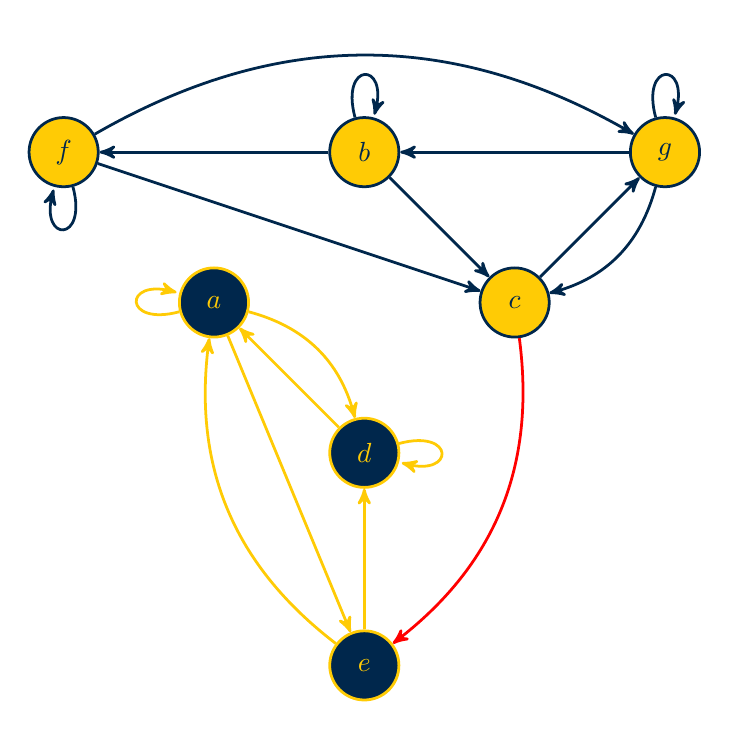
\begin{tikzpicture}[->,>=stealth',auto,node distance=2.7cm,semithick,line width=1pt]
              \tikzstyle{be}=[color=umblue]
              \tikzstyle{me}=[color=ummaize]
              \tikzstyle{re}=[color=red]
              
              \node[state]        (A) [fill=umblue,draw=ummaize,text=ummaize]                  {$a$};
              \node[state]        (B) [above right of=A,fill=ummaize,draw=umblue,text=umblue]  {$b$};
              \node[state]        (D) [below right of=A,fill=umblue,draw=ummaize,text=ummaize] {$d$};
              \node[state]        (C) [below right of=B,fill=ummaize,draw=umblue,text=umblue]  {$c$};
              \node[state]        (F) [above  left of=A,fill=ummaize,draw=umblue,text=umblue]  {$f$};
              \node[state]        (G) [above right of=C,fill=ummaize,draw=umblue,text=umblue]  {$g$};
              \node[state]        (E) [below of=D,fill=umblue,draw=ummaize,text=ummaize]       {$e$};

              \path (A) edge [me,loop  left] node {} (A)
                        edge [me]            node {} (E)
                        edge [me, bend left] node {} (D)
              (F) edge [be,bend  left] node {} (G)
                        edge [be,loop below] node {} (F)
                        edge [be]            node {} (C)
                    (B) edge [be,loop above] node {} (B)
                        edge [be]            node {} (C)
                        edge [be]            node {} (F)
                    (G) edge [be]            node {} (B)
                        edge [be,loop above] node {} (G)
                        edge [be,bend  left] node {} (C)
                    (C) edge [be]            node {} (G)
                        edge [re,bend  left] node {} (E)
                    (D) edge [me,loop right] node {} (D)
                        edge [me]            node {} (A)
                    (E) edge [me,bend  left] node {} (A)
                        edge [me]            node {} (D);
              
       \end{tikzpicture}
       \caption{Example Community Partition}
       \label{fig:ex_comms}
\end{figure}  

\begin{center}
       \begin{tabular}{c|ccccccc} 
              $ \vec{\mathbb{E}} $ & $ a $ & $ b $ & $ c $ & $ d $ & $ e $ & $ f $ & $ g $ \\
              \hline
              $ a $ & $ \frac{9}{15} $ & $ \frac{9}{15} $ & $ \frac{3}{15} $ & $ \frac{6}{15} $ & $ \frac{6}{15} $ & $ \frac{9}{15} $ & $ \frac{9}{15} $ \\
              $ b $ & $ \frac{6}{15} $ & $ \frac{6}{15} $ & $ \frac{2}{15} $ & $ \frac{4}{15} $ & $ \frac{4}{15} $ & $ \frac{6}{15} $ & $ \frac{9}{15} $ \\
              $ c $ & $ \frac{9}{15} $ & $ \frac{9}{15} $ & $ \frac{3}{15} $ & $ \frac{6}{15} $ & $ \frac{6}{15} $ & $ \frac{9}{15} $ & $ \frac{9}{15} $ \\
              $ d $ & $ \frac{9}{15} $ & $ \frac{9}{15} $ & $ \frac{3}{15} $ & $ \frac{6}{15} $ & $ \frac{6}{15} $ & $ \frac{9}{15} $ & $ \frac{9}{15} $ \\
              $ e $ & $ \frac{6}{15} $ & $ \frac{6}{15} $ & $ \frac{2}{15} $ & $ \frac{4}{15} $ & $ \frac{4}{15} $ & $ \frac{6}{15} $ & $ \frac{6}{15} $ \\
              $ f $ & $ \frac{6}{15} $ & $ \frac{6}{15} $ & $ \frac{2}{15} $ & $ \frac{4}{15} $ & $ \frac{4}{15} $ & $ \frac{6}{15} $ & $ \frac{6}{15} $ \\
              $ g $ & $ \frac{9}{15} $ & $ \frac{9}{15} $ & $ \frac{3}{15} $ & $ \frac{6}{15} $ & $ \frac{6}{15} $ & $ \frac{9}{15} $ & $ \frac{9}{15} $ \\
       \end{tabular}
\end{center}

\noindent
Calculating next our inner difference.

\begin{center}
       \begin{tabular}{c|ccccccc} 
              $ \vec{A} - \vec{\mathbb{E}} $ & $ a $ & $ b $ & $ c $ & $ d $ & $ e $ & $ f $ & $ g $ \\
              \hline
              $ a $ & $ \frac{6}{15}  $ & $ \frac{-9}{15} $ & $ \frac{-3}{15} $ & $ \frac{9}{15}  $ & $ \frac{9}{15}  $ & $ \frac{-9}{15} $ & $ \frac{-9}{15} $ \\
              $ b $ & $ \frac{-6}{15} $ & $ \frac{9}{15}  $ & $ \frac{13}{15} $ & $ \frac{-4}{15} $ & $ \frac{-4}{15} $ & $ \frac{9}{15}  $ & $ \frac{-9}{15} $ \\
              $ c $ & $ \frac{-9}{15} $ & $ \frac{-9}{15} $ & $ \frac{-3}{15} $ & $ \frac{-6}{15} $ & $ \frac{9}{15}  $ & $ \frac{-9}{15} $ & $ \frac{6}{15}  $ \\
              $ d $ & $ \frac{6}{15}  $ & $ \frac{-9}{15} $ & $ \frac{-3}{15} $ & $ \frac{9}{15}  $ & $ \frac{-6}{15} $ & $ \frac{-9}{15} $ & $ \frac{-9}{15} $ \\
              $ e $ & $ \frac{9}{15}  $ & $ \frac{-6}{15} $ & $ \frac{-2}{15} $ & $ \frac{11}{15} $ & $ \frac{-4}{15} $ & $ \frac{-6}{15} $ & $ \frac{-6}{15} $ \\
              $ f $ & $ \frac{-6}{15} $ & $ \frac{-6}{15} $ & $ \frac{13}{15} $ & $ \frac{-4}{15} $ & $ \frac{-4}{15} $ & $ \frac{9}{15}  $ & $ \frac{9}{15}  $ \\
              $ g $ & $ \frac{-9}{15} $ & $ \frac{6}{15}  $ & $ \frac{12}{15} $ & $ \frac{-6}{15} $ & $ \frac{-6}{15} $ & $ \frac{-9}{15} $ & $ \frac{6}{15}  $ \\
       \end{tabular}
\end{center}

\noindent
We have our community indication matrix $ \varDelta $.

\begin{center}
       \begin{tabular}{c|ccccccc} 
              $ \varDelta  $ & $ a $ & $ b $ & $ c $ & $ d $ & $ e $ & $ f $ & $ g $ \\
              \hline
              $ a $ & $ 1 $ & $ 0 $ & $ 0 $ & $ 1 $ & $ 1 $ & $ 0 $ & $ 0 $ \\
              $ b $ & $ 0 $ & $ 1 $ & $ 1 $ & $ 0 $ & $ 0 $ & $ 1 $ & $ 1 $ \\
              $ c $ & $ 0 $ & $ 1 $ & $ 1 $ & $ 0 $ & $ 0 $ & $ 1 $ & $ 1 $ \\
              $ d $ & $ 1 $ & $ 0 $ & $ 0 $ & $ 1 $ & $ 1 $ & $ 0 $ & $ 0 $ \\
              $ e $ & $ 1 $ & $ 0 $ & $ 0 $ & $ 1 $ & $ 1 $ & $ 0 $ & $ 0 $ \\
              $ f $ & $ 0 $ & $ 1 $ & $ 1 $ & $ 0 $ & $ 0 $ & $ 1 $ & $ 1 $ \\
              $ g $ & $ 0 $ & $ 1 $ & $ 1 $ & $ 0 $ & $ 0 $ & $ 1 $ & $ 1 $ \\
       \end{tabular}
\end{center}


\noindent
Last $ \vec{Q} = (A - \vec{\mathbb{E}}) : \frac{\varDelta}{m} = 0.42 \overline{6} $.
We would thus consider this graph to exhibits strong community structure with the given partition. 
Due to the small scale of this graph it is easy to identify a good partition, but as networks scale visualization becomes increasingly challenging, and thus such an algorithmic approach as we have outlined is required for analysis. 


\section{Evolution of Algorithms}

Algorithms are most commonly judged on complexity, but there is a clear tradeoff with accuracy (quality). 
Modularity is a proxy metric with the ability to judge the accuracy of a community detection algorithm. 
Traditionally, accuracy is defined with respect to a ground truth, such that the community structure is known within the network, but this information is not always available within a real world dataset. 
Computational complexity is a good reference for scalability of an algorithm, and provides an upper limit on the size of useable networks. 
Additionally as time goes one, Moore's Law realizes, technology improves allowing for denser circuitry. 
A phenomena arises such that the size of usable networks scales proportionally, for algorithms with fixed complexity, to the temporal increase in computational power. 
With that said, for a given dataset, one may be able to execute a more complex algorithm with increased accuracy, in the same run time as a simpler algorithm ran years prior. 
The evolution of algorithms plays on both of these characteristics. 

In the future, we will see networks of ever increasing size. 
Social media networks gain more users; the World Wide Web has new pages added, and links between pages increase. 
Form this perspective, we need to develop algorithms that retain an acceptable accuracy, but are less complex. 
Similarly, we have important networks of which size is relatively stable, for example biological networks such as food webs. 
As a result, algorithms with increased accuracy are of interest, even if they come at a cost of additional run time. 
This dance allows researches to make meaningful insights, whether seeking increased performance in accuracy or complexity. 
Thus often it is the case that previously dismissed works become relevant many years later.  

The first proposal of modularity to the best of our knowledge comes from Newman in \cite{finding_and_evaling_comm_struct}. 
The application was applied to the simplest of networks, undirected and unweighted. 
Modularity was simply used to evaluate goodness of community detection, and impose a stopping condition on a paired detection algorithm. 
Two detection techniques were utilized, both of which utilized edge removal based on a betweenness measure. 
The simpler of the two methods, was to calculate shortest-path betweenness. 
The second method focused on random-walk, or otherwise equivalently current-flow betweenness. 
In both cases, the assumption is that many nodes must supplement flow thorough community-to-community edges. 
In the case of removing these community connecting edges one expects to find the underlying communities, as connected components within the augmented graph. 
In general, the algorithm would be ran until no edges exist. 
After each edge removal, the graphs modularity is calculated. 
The best partition is then selected, such that modularity is maximized.

Depending on the underlying network structure, modularity maximization may yield exactly the opposite of the partitions we seek to find. 
This would happen in the case where the assumption that internal community links should be dense compared to that of external links. 
In the case of disassortative structure, such that links are more dense between communities, rather than within them, we should minimize modularity as previously defined. 
This is equivalent to maximizing $ C_{\% \ external} - C_{\% \ \mathbb{E} \ external} $.
Such an task was initially founded on heuristic grounds, and studied much less than assortative networks. 
It was not until 2016 in \cite{equivalence_between} that Newman game a rigorous explanation of this method when showing the equivalence between modularity optimization and paralleled maximum likelihood estimation methods. 

In a true sense of modularity optimization, one would search all possible partitions of the network and select that which has the best modularity.  
The number of ways to partition a network of $ n $ nodes into $ c $ communities shown in \cite{fast_algorithm} to increase at least exponentially with respect to $ n $, and thus such an exhaustive method is not possible for most all real world networks.
As a result traditional algorithms are only approximations of the maximal modularity, and operate in an iterative manner. 
Thus, modularity is often used as a stopping condition within a method.

It is noticed that there are two forms of which modularity optimization can occur. 
Modularity can be single peaked, such that there is both one global and local maxima. 
Similarly modularity can be multipeaked, such that there is one global but multiple local maxima. 
In either case, one could halt the algorithm after finding the first local maxima. 
In the multipeaked case this halting shall give a `good' partition but not necessarily the best, introducing a probability for reduced accuracy. 
In the single peaked case this technique provides the optimal partition. 
Thus one may opt to impose a halting criteria when and iteration of the community detection algorithm first decreases the graph's modularity.
Clearly, this will reduce the runtime of an algorithm, and is a tradeoff considered by the implementer dependent upon the size of their network, and their accuracy requirement. 

These heuristics form the basis for real world modularity maximization algorithms, and show clearly the tradeoff between complexity and accuracy. 
Algorithms are based on an iterative approach, and in practice if one can drastically reduce complexity, at a slight cost to accuracy, it is preferred. 
In general, implementers seek a good partition of a network into communities, though it may not be the best. 

Historically (pre 2000) algorithms were agglomerative (bottom up), finding communities by the addition of edges rather than removal, such as the well known k-means clustering \cite{least_squares_PCM, some_methods}. 
Newman and Girvan's work shifted the state of the art to decisive (top down) algorithms \cite{com_struct_in_soc_and_bio}, focused on edge removal. 
Soon after Newman's initial work he extended his algorithm to weighted networks \cite{analysis_of_wnets}, thereafter developing an algorithm for modularity maximization, by node joins, reducing complexity \cite{finding_comm_struct} with Clauset and Moore.
Later work by Newman and Leicht extended the algorithm to directed networks \cite{com_struct_indir}, for increased accuracy. 
In parallel Blondel, Guillaume, Lambiotte, and Lefebvre made significant strides in complexity reduction allowing for analysis of massive networks in the 2008 release of the so-called Louvain algorithm \cite{louvain}. 
Their advances leveraged multiple, rather than singular, node joins per iteration by by considering node neighborhoods.
From the perspective of accuracy, Fortunato and Barth{\'{e}}lemy noted early in 2008 a limit to the ability of modularity maximization to find more than $ \sqrt{s} $ communities within networks. 
This showed an underlying issue within the approach at the time, where smaller communities would be joined into larger meta-communities. 
Via a separate quality function, Reichardt and Bornholdt proposed a resolution limit in \cite{statistical_mechanics}, and showed equivalence to historical modularity maximization with set parameters. 
Arenas, Fern{\'{a}}ndez, and G{\'{o}}mez extended soon after extended the resolution parameter to fit within traditional modularity maximization algorithms \cite{different_resolution_levels}. 
Continuing later the Louvain algorithm was extend to directed networks by Dugu{\'{e}} and Perez to account for the additional information provided within the direction of links \cite{directed_louvain}. 
Soon after, Newman showed equivalent of modularity maximization with a special case of log-likelihood maximization under the planted partition stochastic block model respective to initial degree distributions \cite{equivalence_between}. 
Additionally, his paper elaborated upon the optimal value for the resolution parameter, and provided an iterative approach to finding it within the generalized modularity maximization framework. 
This work provided a strong mathematical framework for the method of modularity maximization, rather than a heuristic framework, and pointed out that the model assumes all communities have statistically similar properties, which is not always the case in real world networks.  
Coming to the most recent of developments, the Louvain algorithm was transformed to the Leiden algorithm with an additional reduction in complexity by Traag, Waltman, and van Eck in 2019 \cite{louvain_2_leiden}. 


\section{Analysis of Algorithms}

To consider the run time complexity of any modularity optimization algorithm we must first consider the requirement for computing modularity alone. 
First, let us assume the only data structure we have is an array containing an adjacency matrix of the network under consideration. 
Next, let our first calculation be $ s $ the total number of spokes within the network. 
Doing so is a sum across all entries in the adjacency matrix, and takes $ n^{2} $ retrievals, followed by $ n^{2} -1 $ additions, a total of $ 2n^{2} $ operations.
We will assume this step happens during matrix initialization, and thus consider insertions rather than retrievals. 
Thus, the calculation of $ s $, or otherwise $ m = s/2 $, runs in time $ \mathcal{O}(n^{2}) $. 
In order to compute the degree, or otherwise in/out-degree, of a node, we must sum row/column-wise for each node. 
Each summation requires $ n $ retrievals, followed by $ n - 1 $ additions, a total of $ 2n -1 $ operations, with complexity $ \mathcal{O}(n) $.
Retrieving the true number of edges between two nodes, as well as a single subtraction or multiplication happens in constant time $ \mathcal{O}(1) $. 
In a naive implementation, we would calculate $ A_{i, j} - E_{i, j} $ for each node pair $ i, j $.
Such a method would require $ n^{2} $ calculations, later followed by $ n^{2} - 1 $ additions, disregarding the computational requirement for finding $ \delta(c_{i}, c_{j}) $. 
This runs in time $ \mathcal{O}(n^{2}) $, and thus our total complexity for computing modularity would be $ \mathcal{O}(n^{2} + n^{2}(n)) = \mathcal{O}(n^{3}) $.
Rather this is not the case, but in practice networks are initialized with each node existing in a sole community, and thus we can see $ \delta(c_{i}, c_{j}) = 1 $ only when $ i = j $, and can operate under the assumption that modularity is as follows. 

\begin{flalign*}
       & \ds \vec{Q}(\gamma) = \frac{1}{m} \sum_{i}^{n} \left( \vec{A}_{i, i} - \gamma \frac{k_{i}^{in} k_{i}^{out}}{m} \right)
\end{flalign*}

\noindent
We need only compute the inner value of our sum $ n $ times, and can operate in complexity $ \mathcal{O}(n^{2} + n(n)) = \mathcal{O}(n^{2}) $.
We can now see that the initialization of the algorithm alone can be quite costly for large networks. 

Let us now lay down a traditional greedy algorithm for further analysis. 
Such an algorithm can be explained in the following five steps. 

\begin{enumerate}
       \item Initialize your adjacency matrix $ A $ and compute $ s, m $.
       \item For each edge, consider the change in modularity $ (\Delta Q) $ given it was to be removed, and the nodes on each side of it joined. 
       \item Join the two nodes with the largest positive value for $ \Delta Q $, to form a new adjacency matrix $ A' $.
       \item Store the community assignments and modularity for the given iteration.
       \item Repeat steps $ 2,3,4 $ on $ A' $ until all node joins are exhausted, and select to community distribution corresponding to the larges value of $ Q $.
\end{enumerate}

\noindent
After obtaining initial modularity we can compute the modularity of $ A' $ in $ \mathcal{O}(n^{2}) $ time. In order to do so we may first compute $ A' $ given we join the node pair corresponding to the edge removal, and if this new graph has the highest modularity change seen yet cache it, along with $ \Delta Q $. 
$ A' $ has 1 less column and 1 less row than $ A $, in fact, the only change is that the 2 nodes which are joined have their rows/columns replaced with their sum. 
The operation takes at most $ 4n -2 $ retrievals and $ 2n - 1 $ additions, happening in $ \mathcal{O}(n) $. 
What we can now see is that calculating $ \Delta Q $ happens in time $ \mathcal{O}(n + n^{2}) = \mathcal{O}(n^{2})$
With that said, the first iteration, and thus the worst case, of the algorithm requires we do so for each and every edge, which means finding the best edge to remove, and thus the best $ A' $ to use as a new base, happens in time $ \mathcal{O}(mn^{2}) $.
If we run this algorithm without any stopping condition, we must perform $ n - 1 $ joins, ending in one single node representing the graph as a whole, encompassed as the only community. 
This algorithm is the most basic approach to modularity maximization, and runs in time $ \mathcal{O}(mn^{3}) $.
There are many clever ticks an implementer can do to increase the speed of such an algorithms, which were hinted at in section \textbf{4}, and are available in the cited readings. 


\section{Conclusion}

In this discussion we have identified basics of networks, reviewed the mechanics of disjoint community detection within network, and discussed the history of community detection algorithms. 
Future work shall include an analysis of the more advanced algorithms aforementioned, providing deeper insights into the relevance of historical advancements. 
Additional work permits review of overlapping community detection algorithms, along with their sequential development. 
Worth while is to weight the pros and cons of disjoint vs. overlapping algorithms. 
As computational power and datasets grow, an understanding of where we come from is crucial to proper implementation and selection of cutting edge network algorithms.



\bibliography{draftfinal.bib}{}
\bibliographystyle{acm} % abbrv, acm, alpha, apalike, ieeetr, plain, siam, unsrt

\end{document}